\section{R-CNN Family}
\begin{frame}{}
    \LARGE Object Detection: \textbf{R-CNN Family}
\end{frame}

\begin{frame}[allowframebreaks]{R-CNN Family}
    \begin{figure}
        \centering
        \fetchconvertimage{https://lilianweng.github.io/posts/2017-12-31-object-recognition-part-3/rcnn-family-summary.png}{images/object-detect/r-cnn-family.png}{width=\textwidth,height=0.9\textheight,keepaspectratio}
    \end{figure}

    \framebreak

    \begin{enumerate}
        \setlength{\itemsep}{1em}
        \item \textbf{R-CNN}: Uses selective search to propose regions, then classifies each region using a CNN.
        \item \textbf{Fast R-CNN}: Improves R-CNN by sharing computation across regions, using a single CNN for the entire image.
        \item \textbf{Faster R-CNN}: Introduces a Region Proposal Network (RPN) to generate region proposals, making it faster and more efficient.
        \item \textbf{Mask R-CNN}: Extends Faster R-CNN to also predict segmentation masks for each detected object.
    \end{enumerate}
\end{frame}


\subsection{R-CNN}
\begin{frame}{}
    \LARGE Object Detection: \textbf{Regions with Convolutional Neural Networks (R-CNN)}
\end{frame}

\begin{frame}[allowframebreaks]{R-CNN}
    \begin{itemize}
        \item \textbf{R-CNN} stands for \textit{Regions with Convolutional Neural Networks}.
        \item Proposed by Ross Girshick et al. in 2014.
        \item Combines region proposals with CNNs for object detection.
        \item Steps:
        \begin{enumerate}
            \item Generate region proposals (e.g., using Selective Search).
            \item Warp each region and extract features using a CNN.
            \item Classify each region and refine bounding boxes.
        \end{enumerate}
        \item Achieved significant improvements over traditional methods (e.g., sliding windows, hand-crafted features).
    \end{itemize}

\framebreak

    \begin{figure}
        \centering
        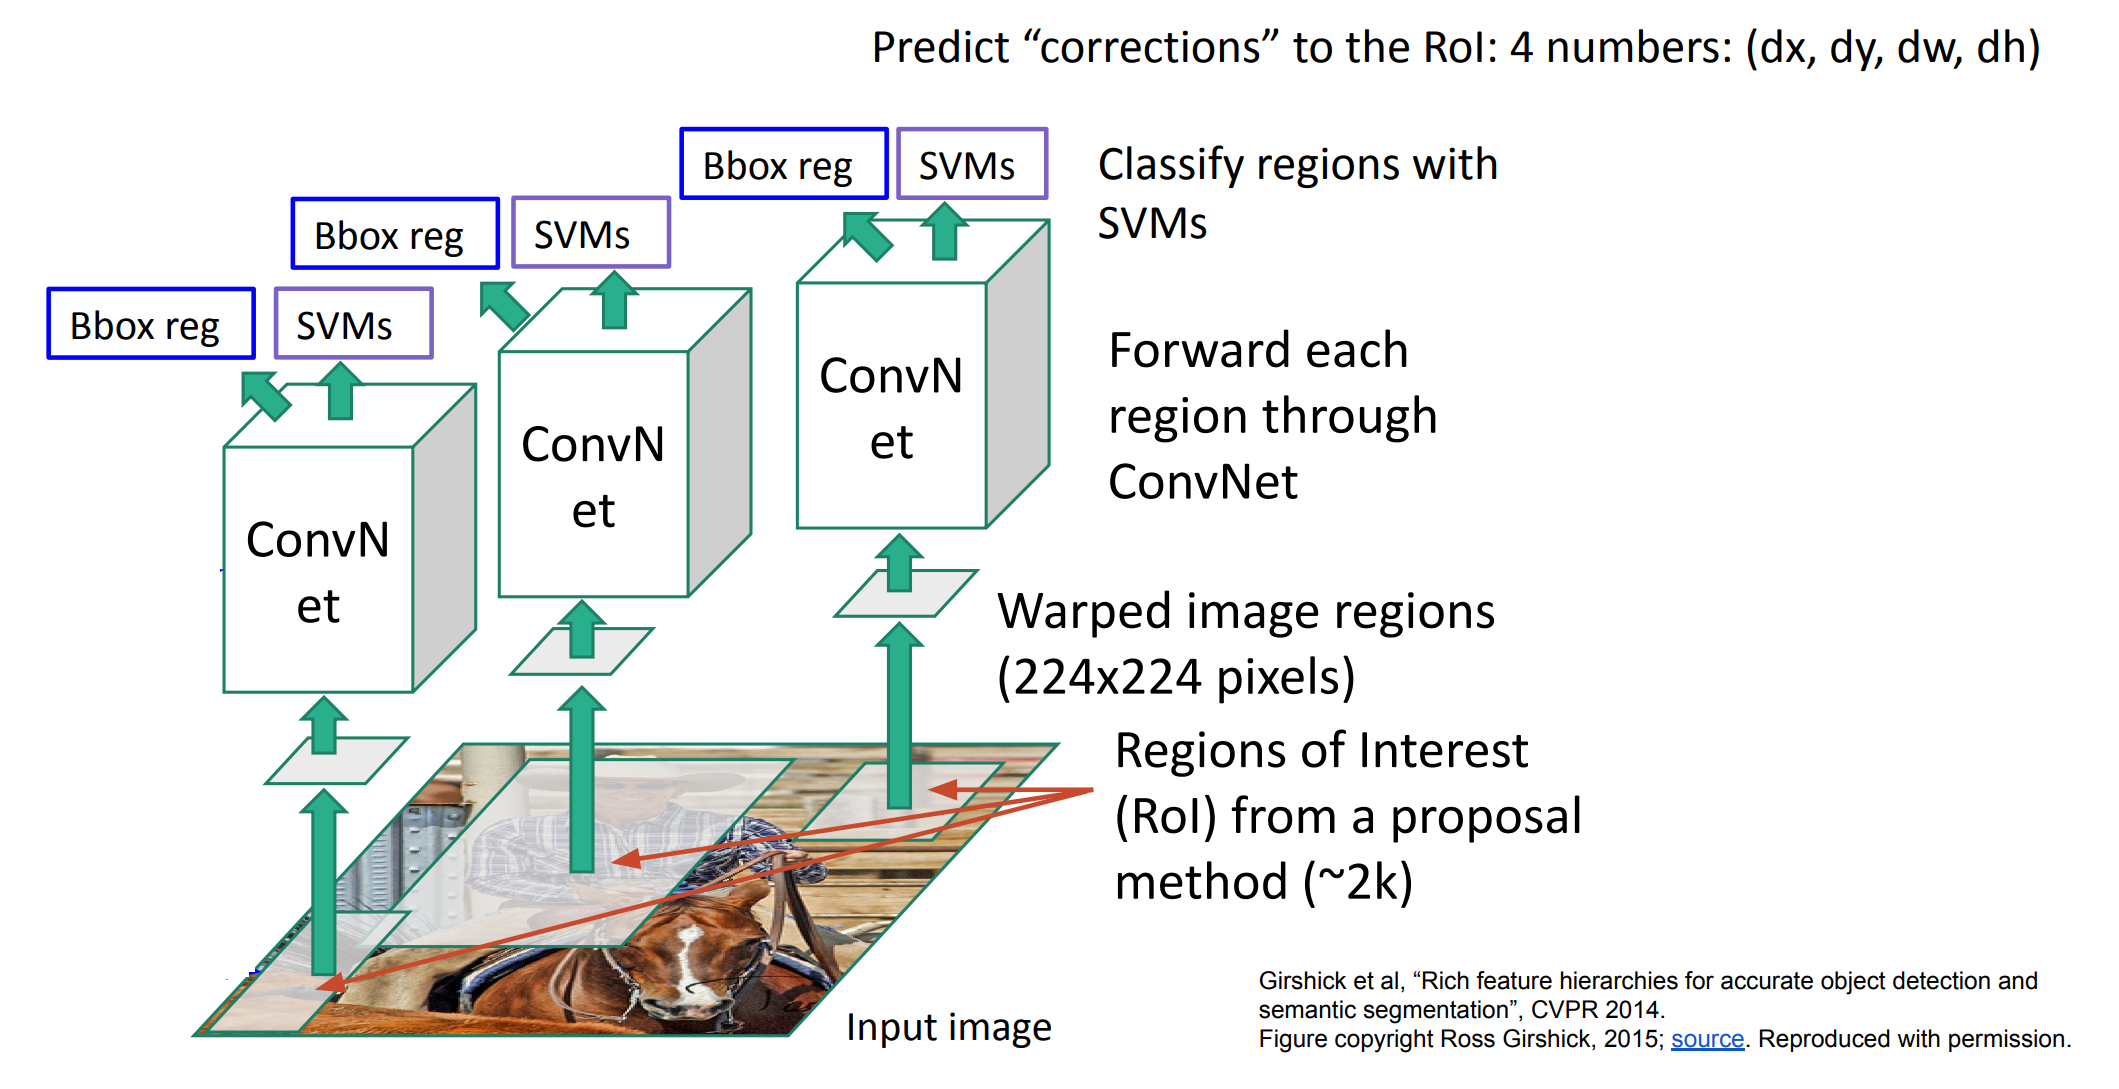
\includegraphics[width=1.0\textwidth,height=1.0\textheight,keepaspectratio]{images/object-detect/rcnn_1.png}
    \end{figure}

\framebreak

    \large R-CNN follows a \textbf{three-step pipeline} for object detection:
        \begin{enumerate}
            \item \textbf{Region Proposal (Selective Search)}
            \begin{itemize}
                \item Instead of using a brute-force sliding window approach, R-CNN applies \textbf{Selective Search}, an algorithm that identifies around \textbf{2000 candidate object regions} (called region proposals).
                \item This significantly reduces the number of regions to process, making the model more efficient.
            \end{itemize}
            \begin{figure}
                \centering
                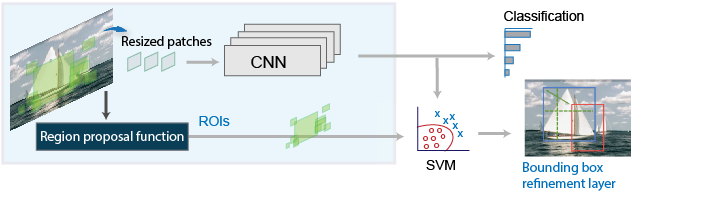
\includegraphics[width=1.0\textwidth,height=0.4\textheight,keepaspectratio]{images/object-detect/r-cnn-region-proposal.png}
            \end{figure}
\framebreak
            \item \textbf{Feature Extraction with CNN}
            \begin{itemize}
                \item Each region proposal is cropped from the image and resized to a fixed size (e.g., 224x224 pixels).
                \item The cropped regions are passed through a \textbf{pre-trained CNN} (like AlexNet or VGG16) to extract deep features.
                \item These features are then stored for classification.
            \end{itemize}
            \begin{figure}
                \centering
                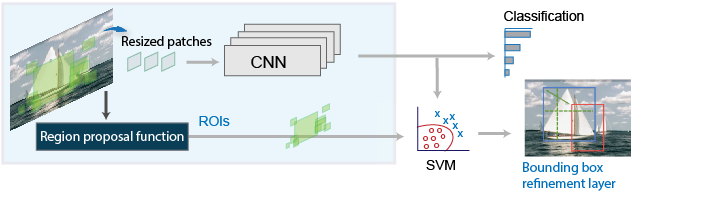
\includegraphics[width=1.0\textwidth,height=0.4\textheight,keepaspectratio]{images/object-detect/r-cnn-region-proposal.png}
            \end{figure}
\framebreak
            \item \textbf{Object Classification \& Bounding Box Refinement}
            \begin{itemize}
                \item The extracted features are passed through a \textbf{Support Vector Machine} (SVM) classifier to determine the object category.
                \item A \textbf{bounding box regression} model is used to fine-tune the position of the detected objects.
            \end{itemize}
            \begin{figure}
                \centering
                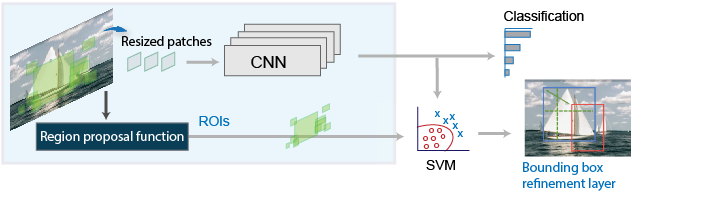
\includegraphics[width=1.0\textwidth,height=0.4\textheight,keepaspectratio]{images/object-detect/r-cnn-region-proposal.png}
            \end{figure}
        \end{enumerate}

\framebreak

        \begin{figure}
            \centering
            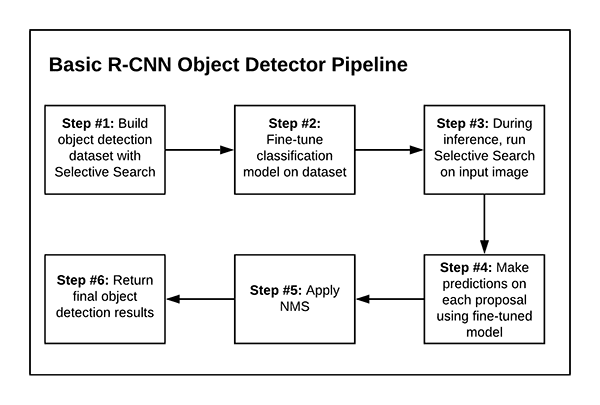
\includegraphics[width=1.0\textwidth,height=0.9\textheight,keepaspectratio]{images/object-detect/r-cnn-pipeline.png}
        \end{figure}
\end{frame}

\begin{frame}[allowframebreaks]{R-CNN: Problem}
    \begin{figure}
        \centering
        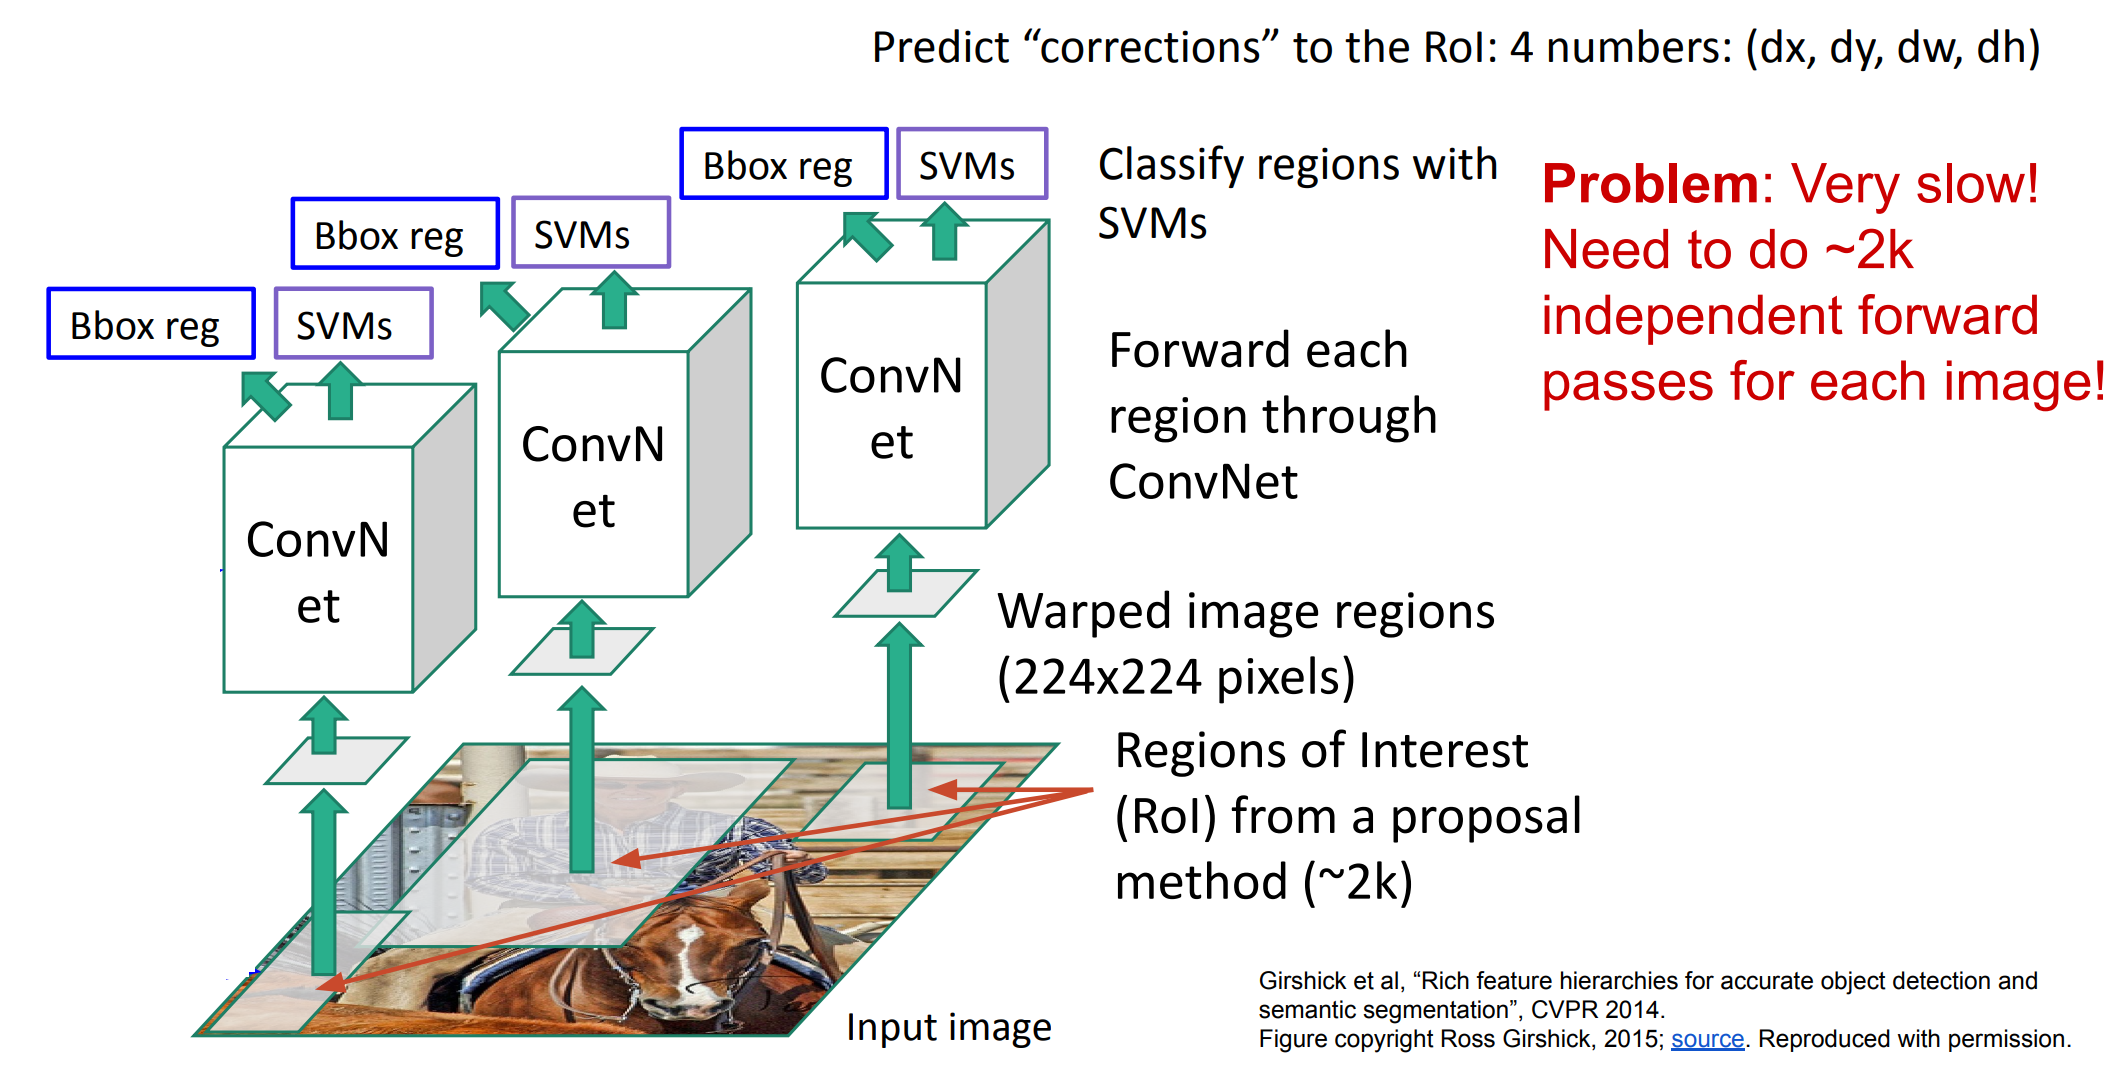
\includegraphics[width=1.0\textwidth,height=1.0\textheight,keepaspectratio]{images/object-detect/rcnn_2.png}
    \end{figure}

\framebreak

    \begin{figure}
        \centering
        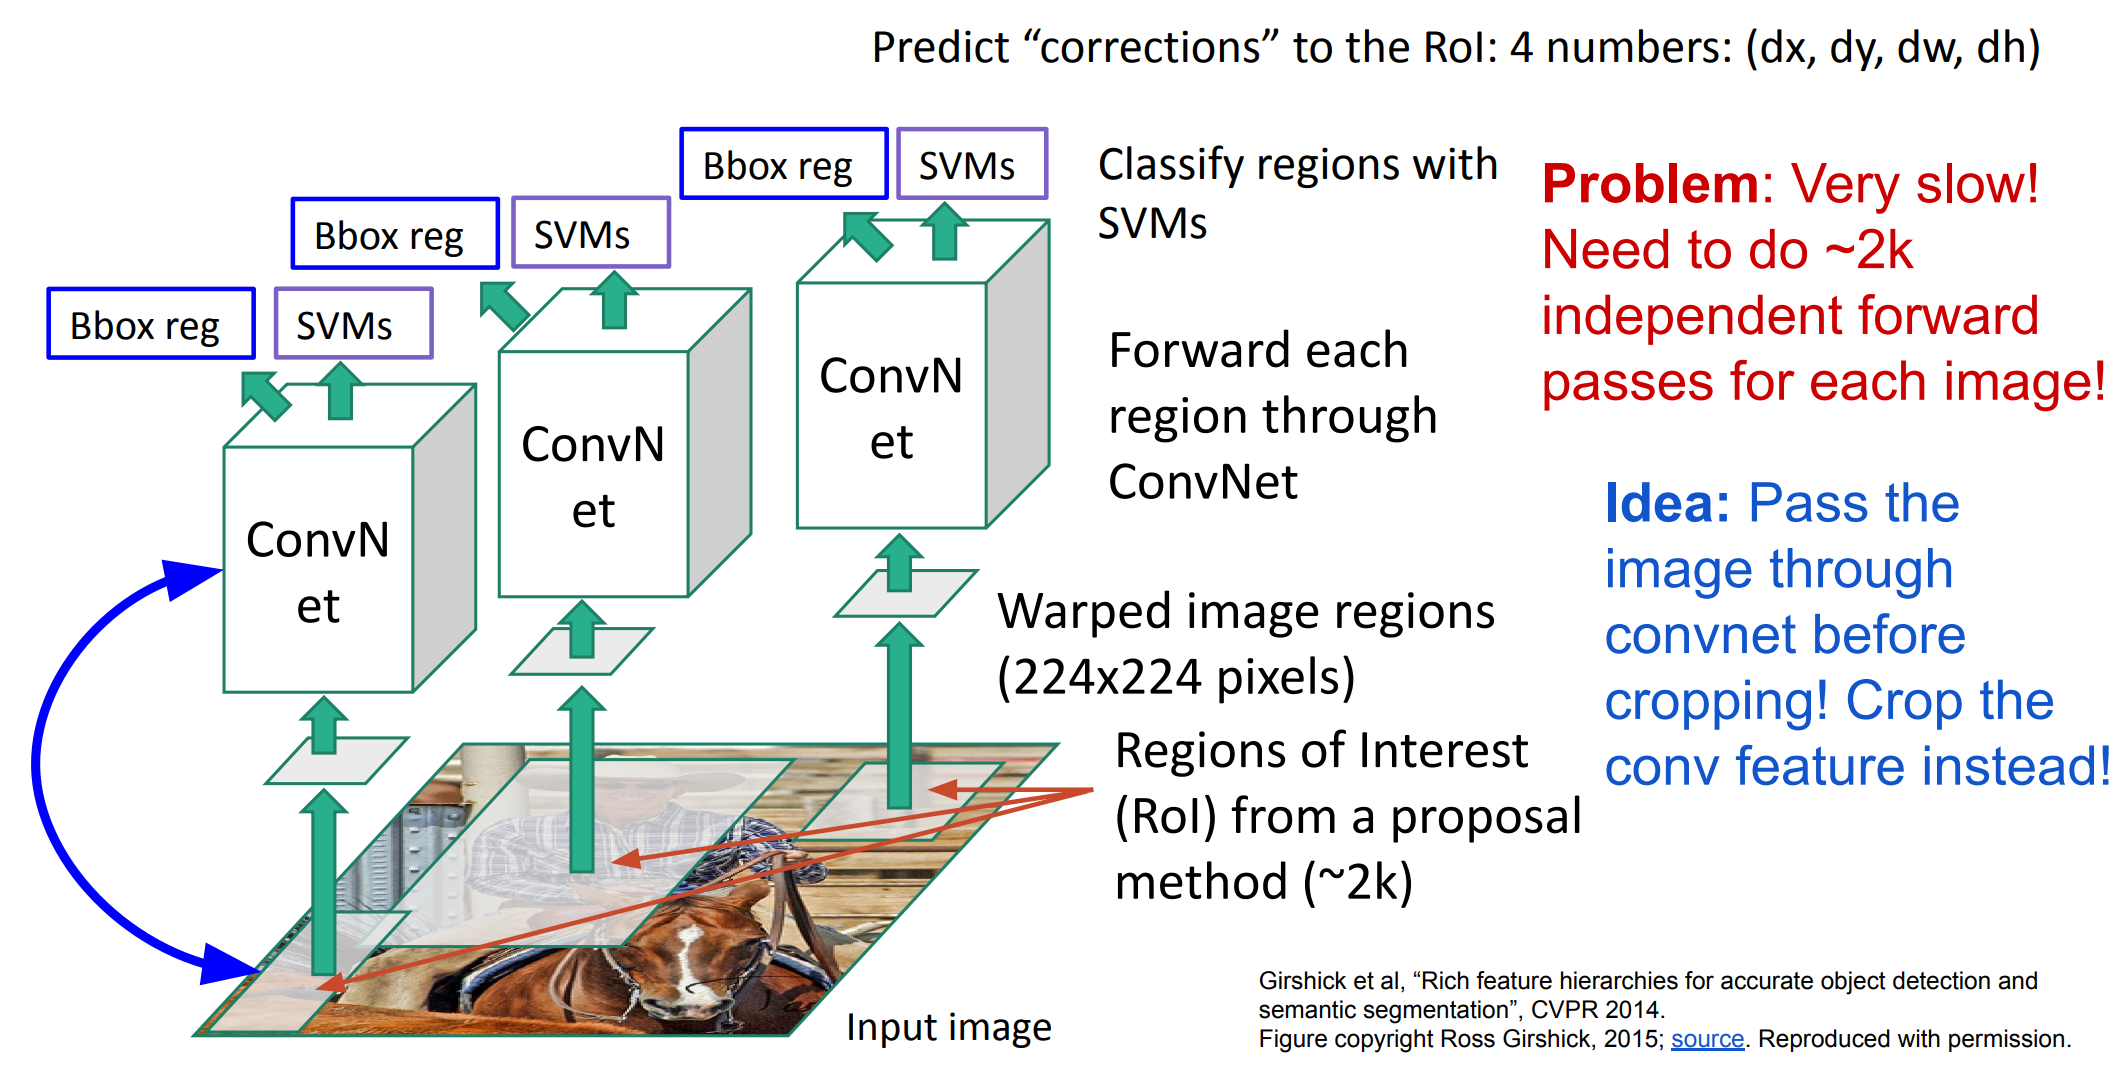
\includegraphics[width=1.0\textwidth,height=1.0\textheight,keepaspectratio]{images/object-detect/rcnn_3.png}
    \end{figure}
\end{frame}

\begin{frame}{Evolution of R-CNN}
    \begin{itemize}
        \item \textbf{R-CNN} inspired a series of improved models:
        \begin{itemize}
            \item \textbf{Fast R-CNN}: Performs feature extraction for all region proposals in a single forward pass, greatly increasing speed and efficiency.
            \item \textbf{Faster R-CNN}: Introduces a \textbf{Region Proposal Network (RPN)} to generate region proposals, making the process end-to-end and even faster.
            \item \textbf{Mask R-CNN}: Extends Faster R-CNN by adding a branch for predicting segmentation masks, enabling instance segmentation.
        \end{itemize}
        \item These advancements have made deep learning-based object detection both faster and more accurate.
    \end{itemize}
\end{frame}
\subsection{Fast R-CNN}
\begin{frame}{}
    \LARGE Object Detection: \textbf{Fast R-CNN}
\end{frame}

\begin{frame}{Fast R-CNN}
    \begin{figure}
        \centering
        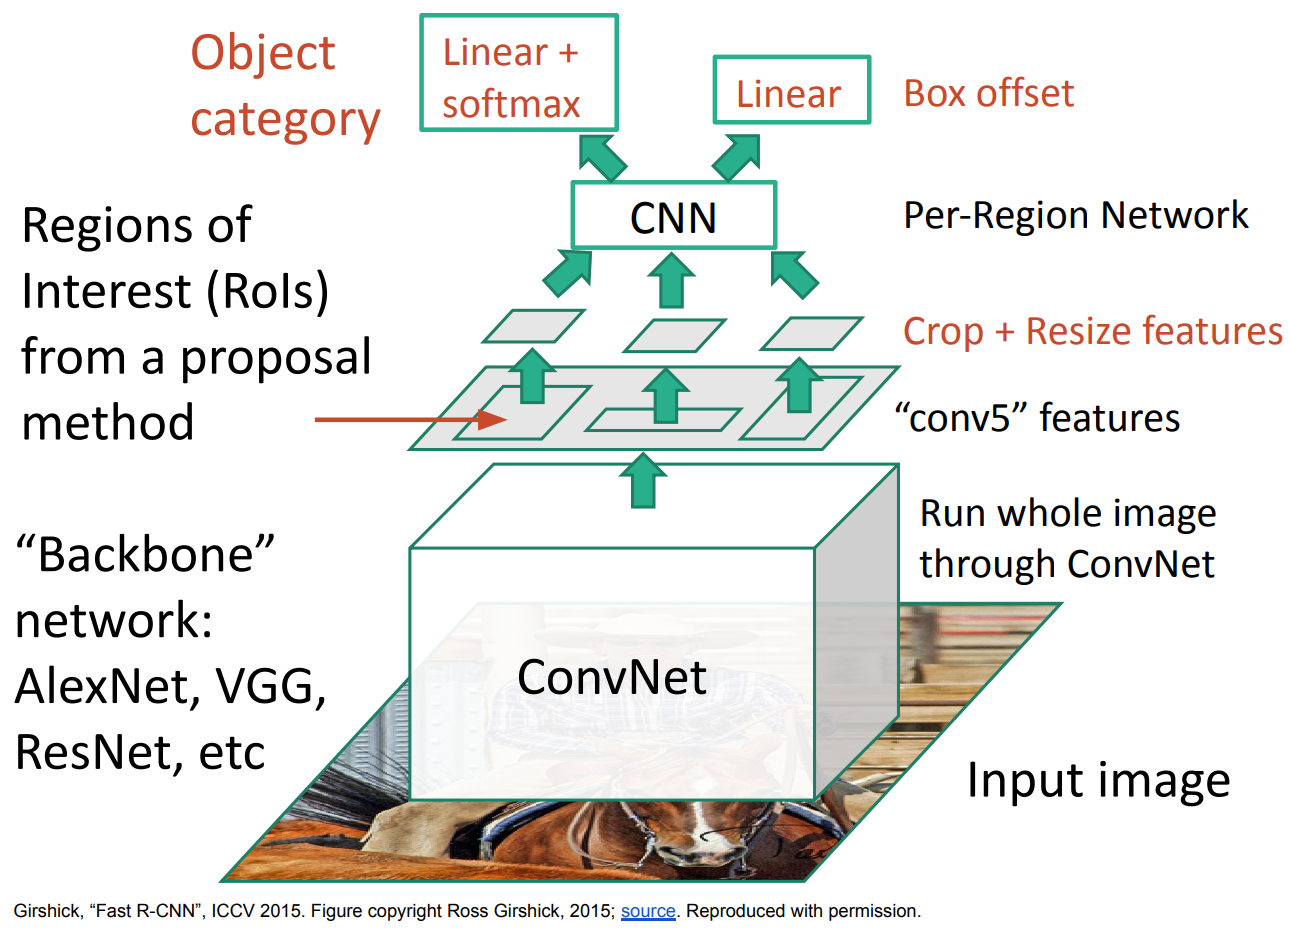
\includegraphics[width=1.0\textwidth,height=1.0\textheight,keepaspectratio]{images/object-detect/fast_rcnn_1.png}
    \end{figure}

\framebreak

    \begin{figure}
        \centering
        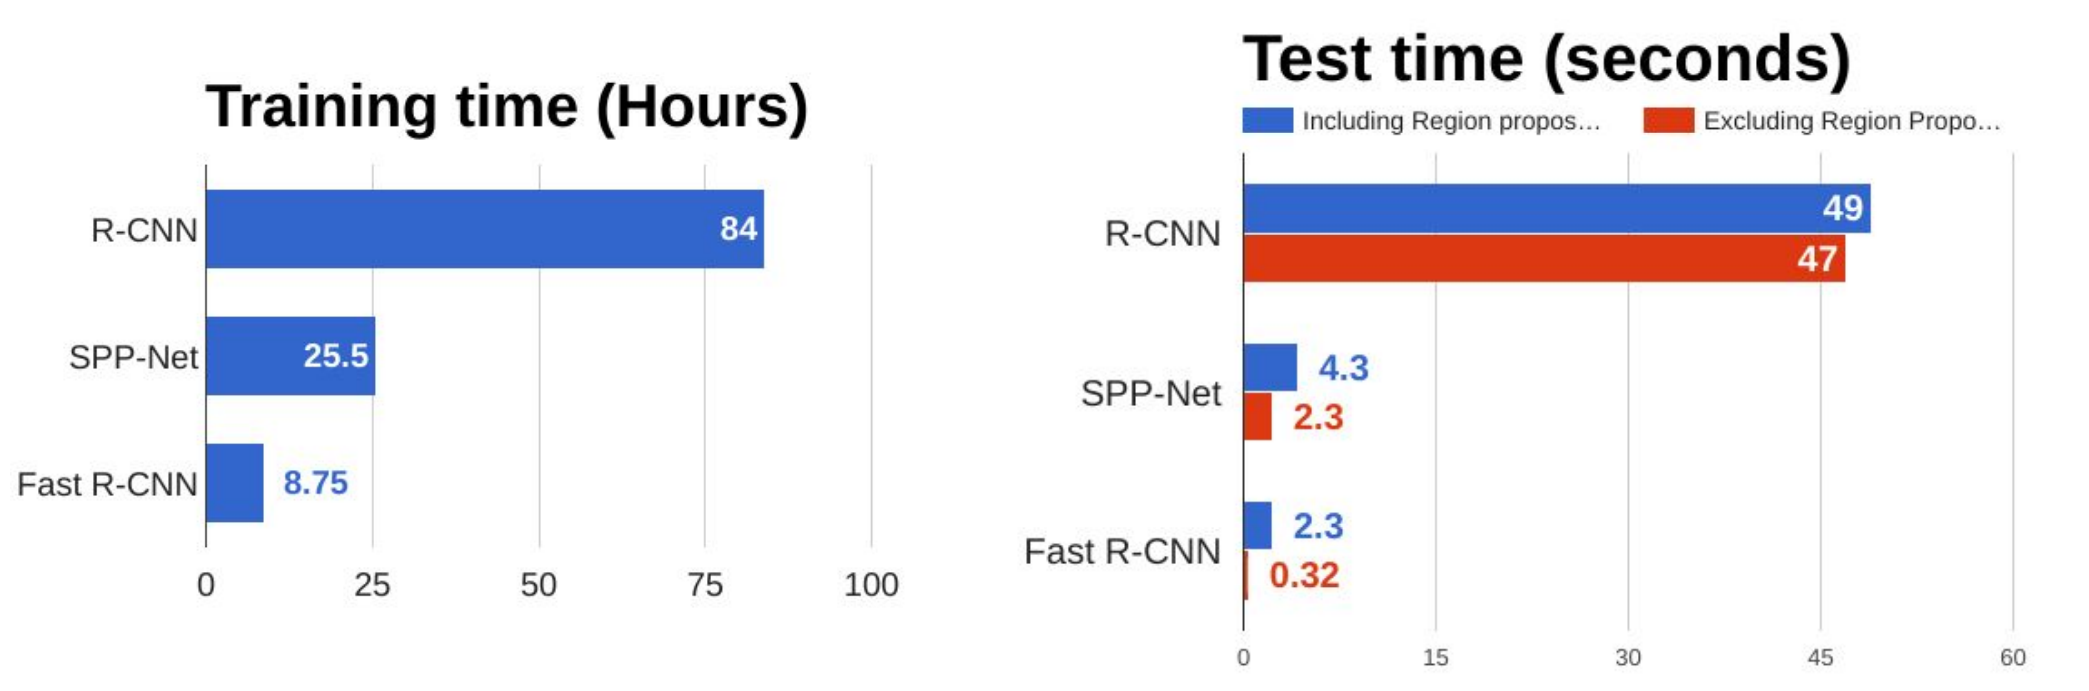
\includegraphics[width=1.0\textwidth,height=1.0\textheight,keepaspectratio]{images/object-detect/fast_rcnn_2.png}
    \end{figure}

\framebreak

    \begin{figure}
        \centering
        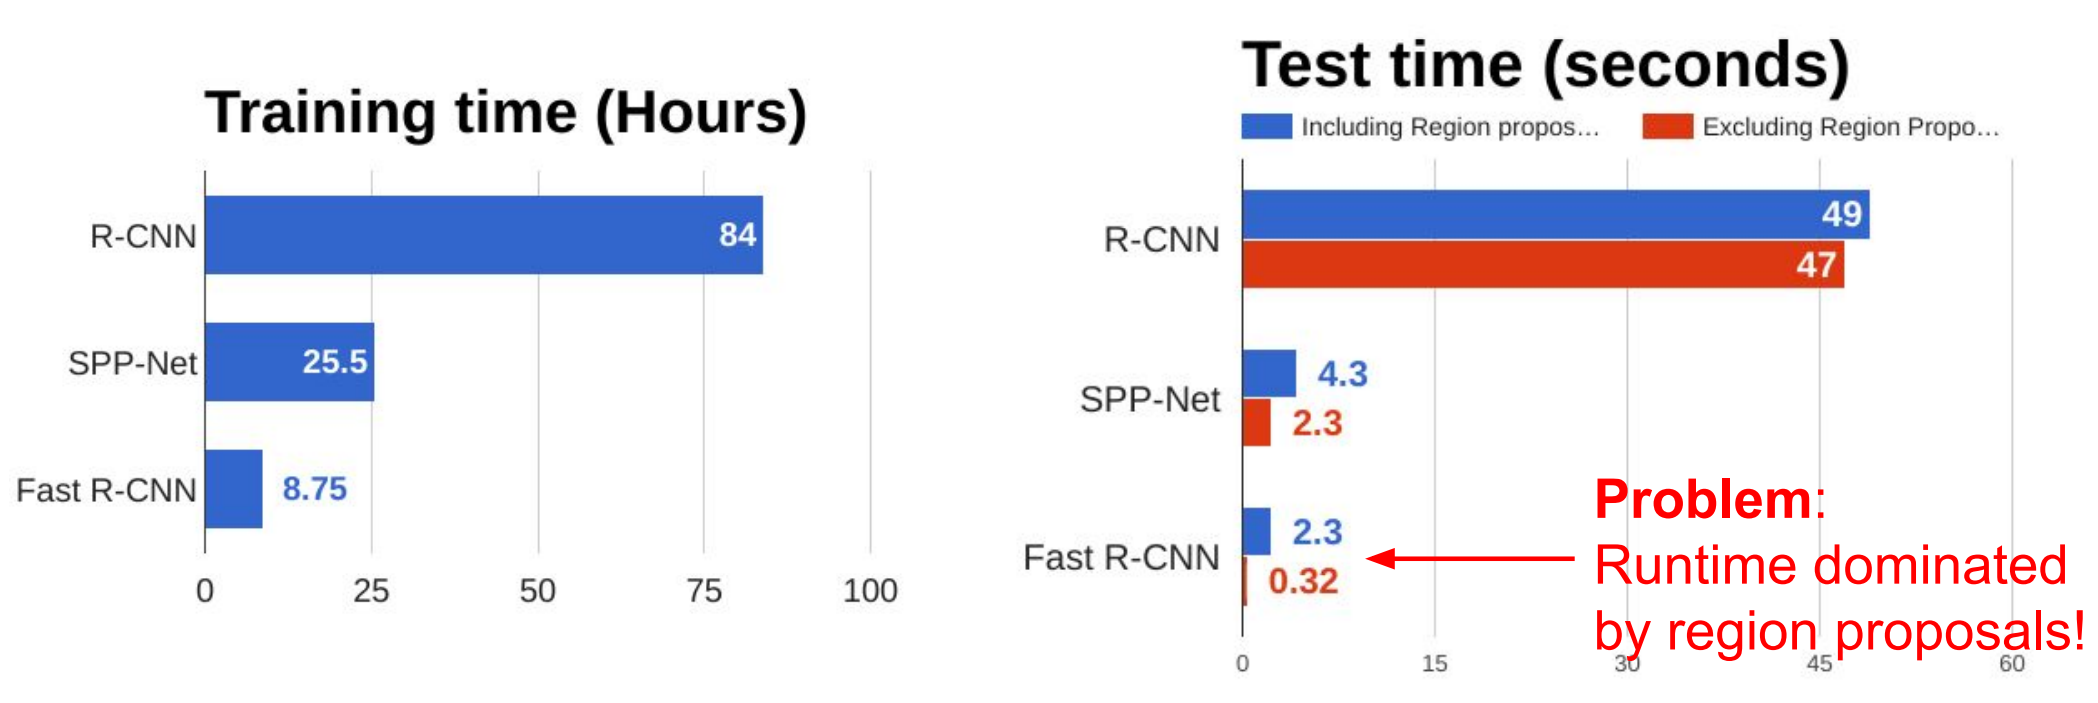
\includegraphics[width=1.0\textwidth,height=1.0\textheight,keepaspectratio]{images/object-detect/fast_rcnn_3.png}
    \end{figure}
    
\end{frame}
\subsection{Faster R-CNN}
\begin{frame}{}
    \LARGE Object Detection: \textbf{Faster R-CNN}
\end{frame}

\begin{frame}{Faster R-CNN}
    \begin{itemize}
        \item Make CNN do proposals!
        \item Insert Region Proposal Network (RPN) to predict proposals from features
        \pause
        \item Jointly train on 4 losses:
        \begin{itemize}
            \item \textbf{RPN classification:} anchor box is object / not an object
            \item \textbf{RPN regression:} predict transform from anchor box to proposal box
            \item \textbf{Object classification:} classify proposals as background / object class
            \item \textbf{Object regression:} predict transform from proposal box to object box
        \end{itemize}
    \end{itemize}
    
\end{frame}

\begin{frame}[allowframebreaks]{Faster R-CNN}
    \begin{figure}
        \centering
        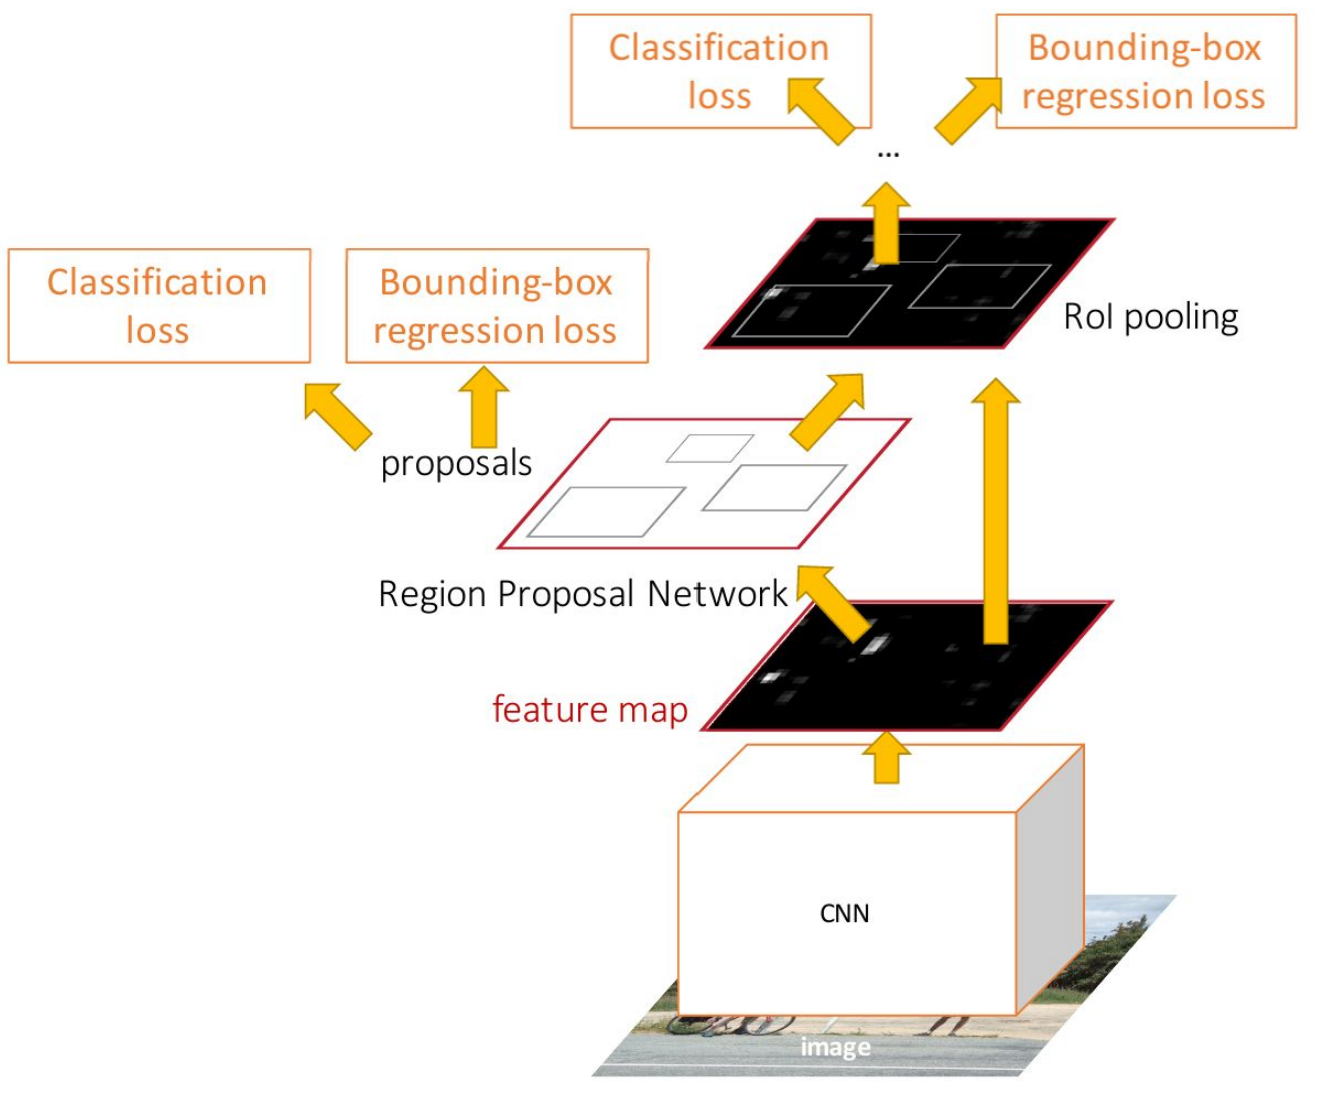
\includegraphics[width=1.0\textwidth,height=0.9\textheight,keepaspectratio]{images/object-detect/faster_rcnn_1.png}
    \end{figure}

\framebreak

    \begin{figure}
        \centering
        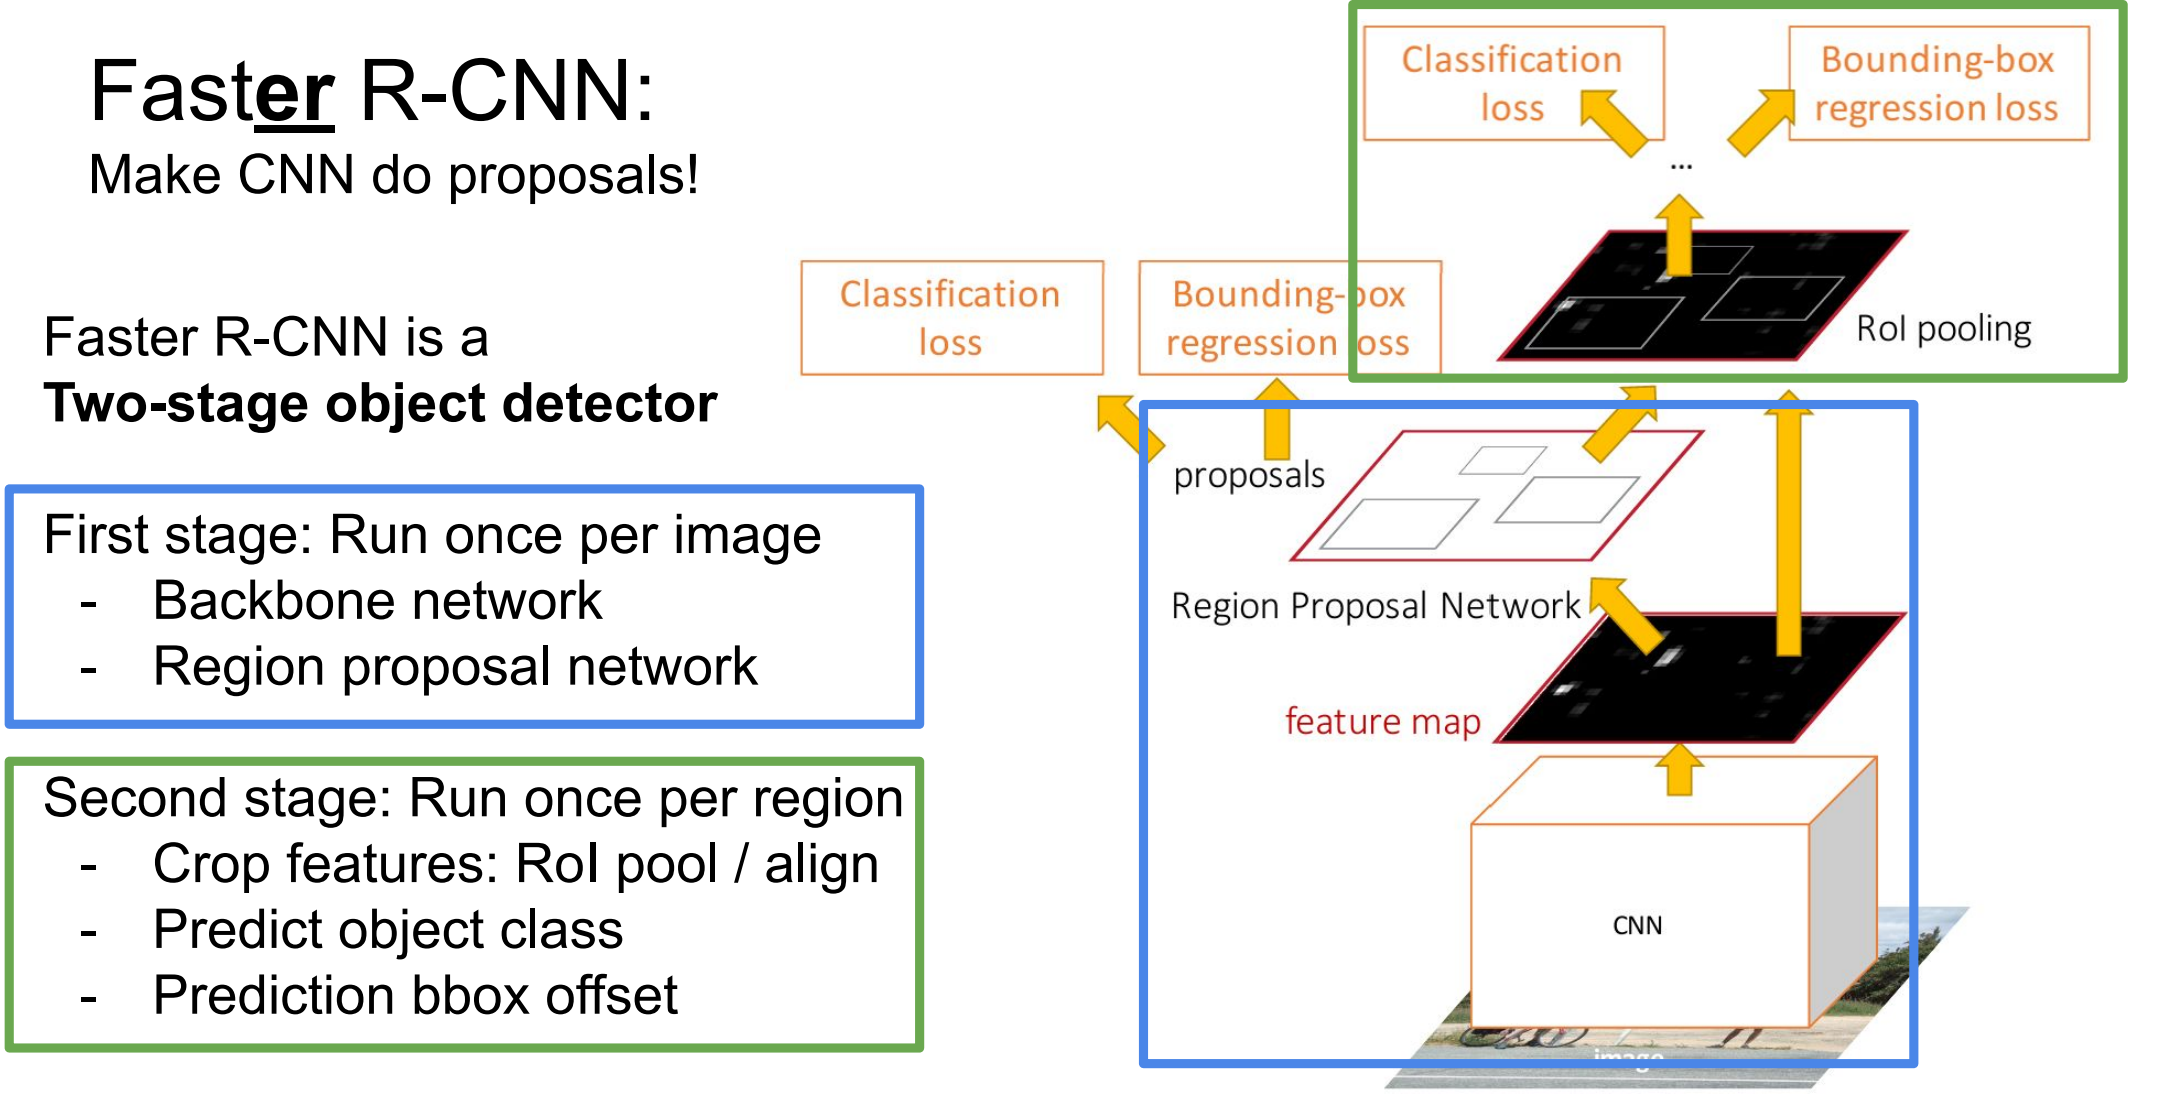
\includegraphics[width=1.0\textwidth,height=1.0\textheight,keepaspectratio]{images/object-detect/faster_rcnn_2.png}
    \end{figure}

\framebreak

    \begin{figure}
        \centering
        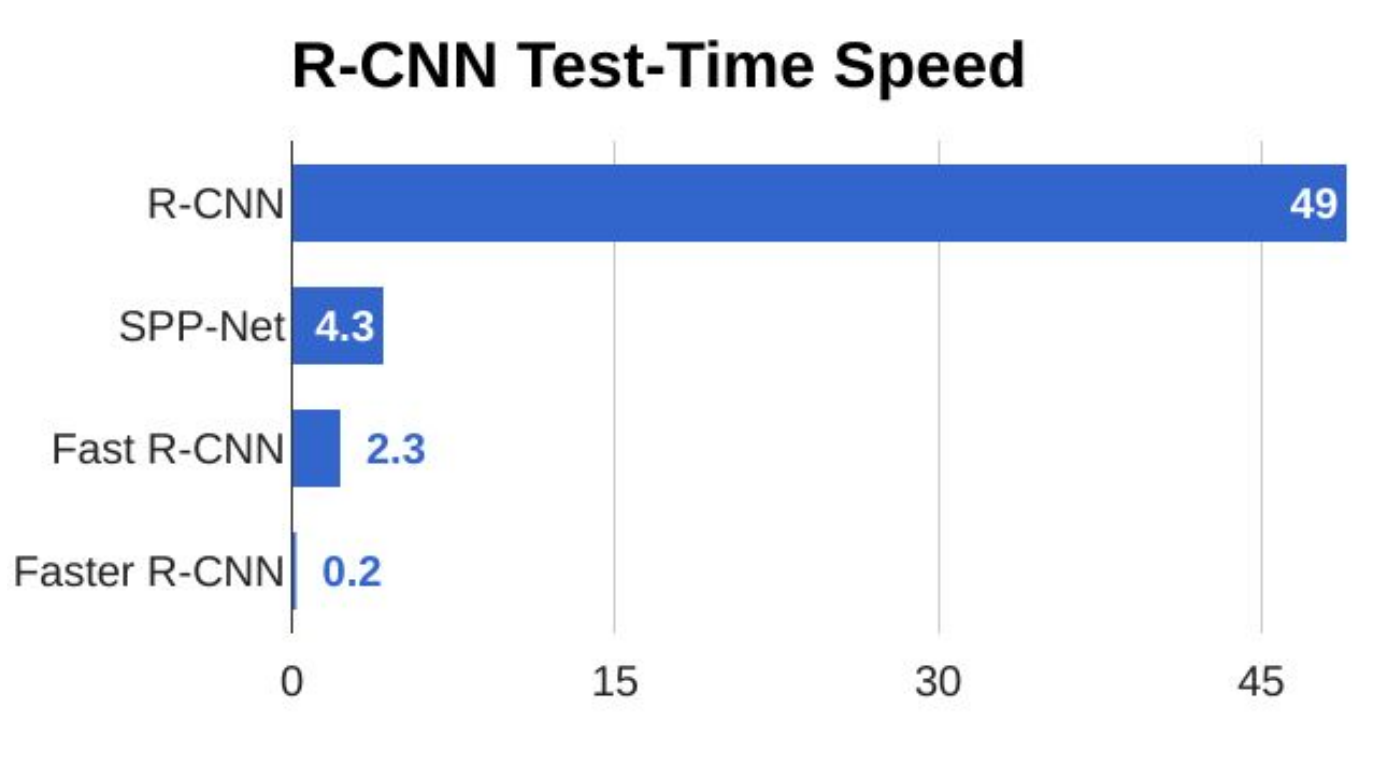
\includegraphics[width=1.0\textwidth,height=1.0\textheight,keepaspectratio]{images/object-detect/faster_rcnn_3.png}
    \end{figure}
\end{frame}
\subsection{Mask R-CNN}
\begin{frame}{}
    \LARGE Instance Segmentation: \textbf{Mask R-CNN}
\end{frame}

\begin{frame}[allowframebreaks]{Mask R-CNN}
    \textbf{Mask R-CNN Overview}
    \begin{itemize}
        \item \textbf{Developed on top of Faster R-CNN}
        \item Faster R-CNN outputs:
        \begin{itemize}
            \item Class label
            \item Bounding-box offset
        \end{itemize}
        \item Mask R-CNN adds a third branch:
        \begin{itemize}
            \item Predicts object mask for each candidate
        \end{itemize}
        \item Performs both \textbf{Semantic} and \textbf{Instance Segmentation}
    \end{itemize}

\framebreak

    \only<1>{
        \begin{figure}
        \centering
        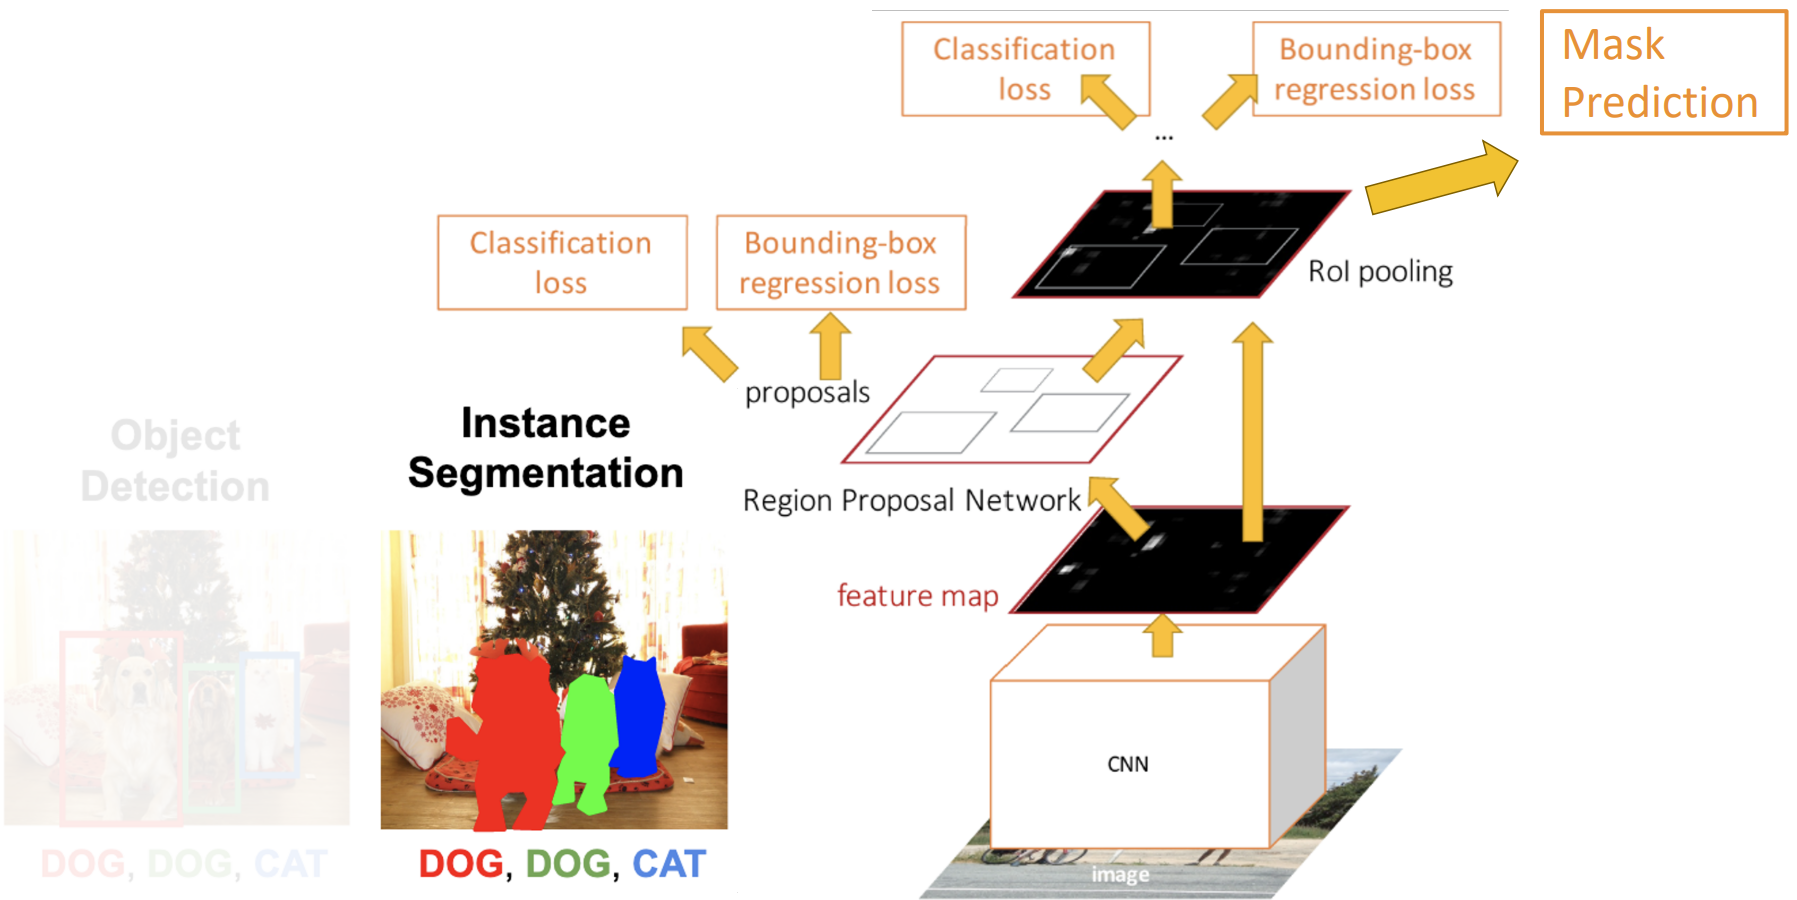
\includegraphics[width=1.0\textwidth,height=1.0\textheight,keepaspectratio]{images/object-detect/ins_6.png}
        \footnotetext{He et al, “Mask R-CNN”, ICCV 2017}
        \end{figure}
    }
    
    \only<2>{
        \begin{figure}
        \centering
        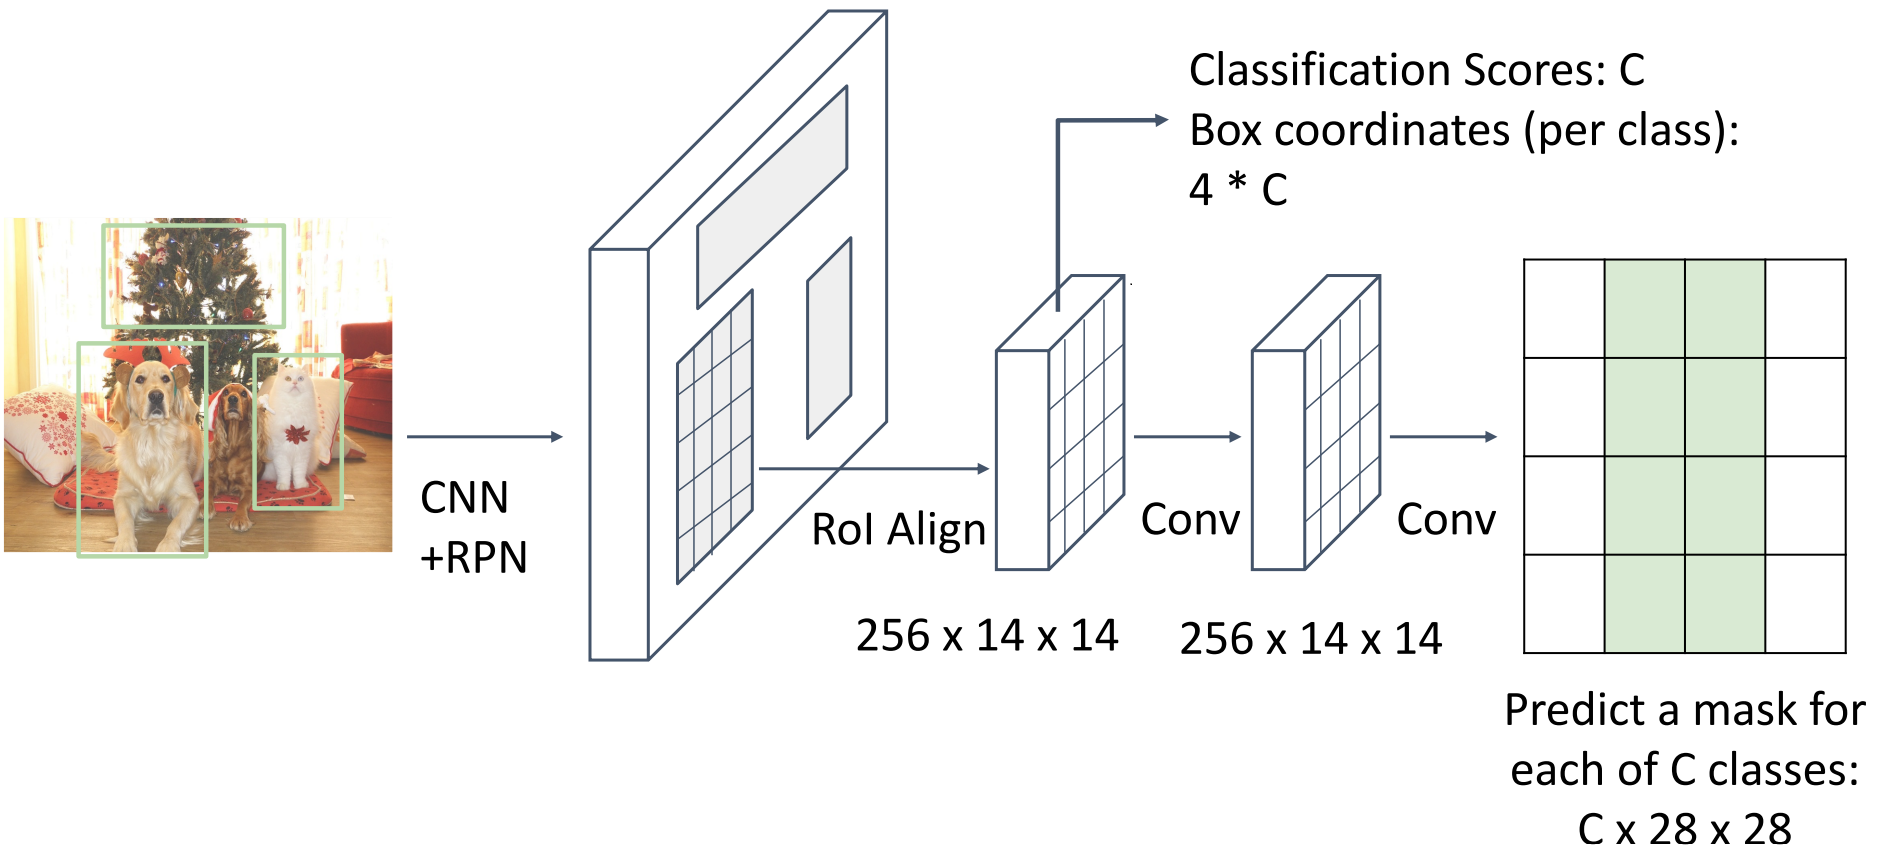
\includegraphics[width=1.0\textwidth,height=1.0\textheight,keepaspectratio]{images/object-detect/ins_7.png}
        \end{figure}
    }

\framebreak

    \textbf{Advantages of Mask R-CNN}
    \begin{itemize}
        \item \textbf{Simplicity}: Simple to train
        \item \textbf{Performance}: Outperforms previous methods, works almost in real-time
        \item \textbf{Efficiency}: Very efficient, small overhead compared to Faster R-CNN
        \item \textbf{Flexibility}: Can perform detection and estimation tasks simultaneously
    \end{itemize}
\end{frame}

\begin{frame}{Mask R-CNN: Example Training Targets}
    \only<2>{
        \begin{figure}
            \centering
            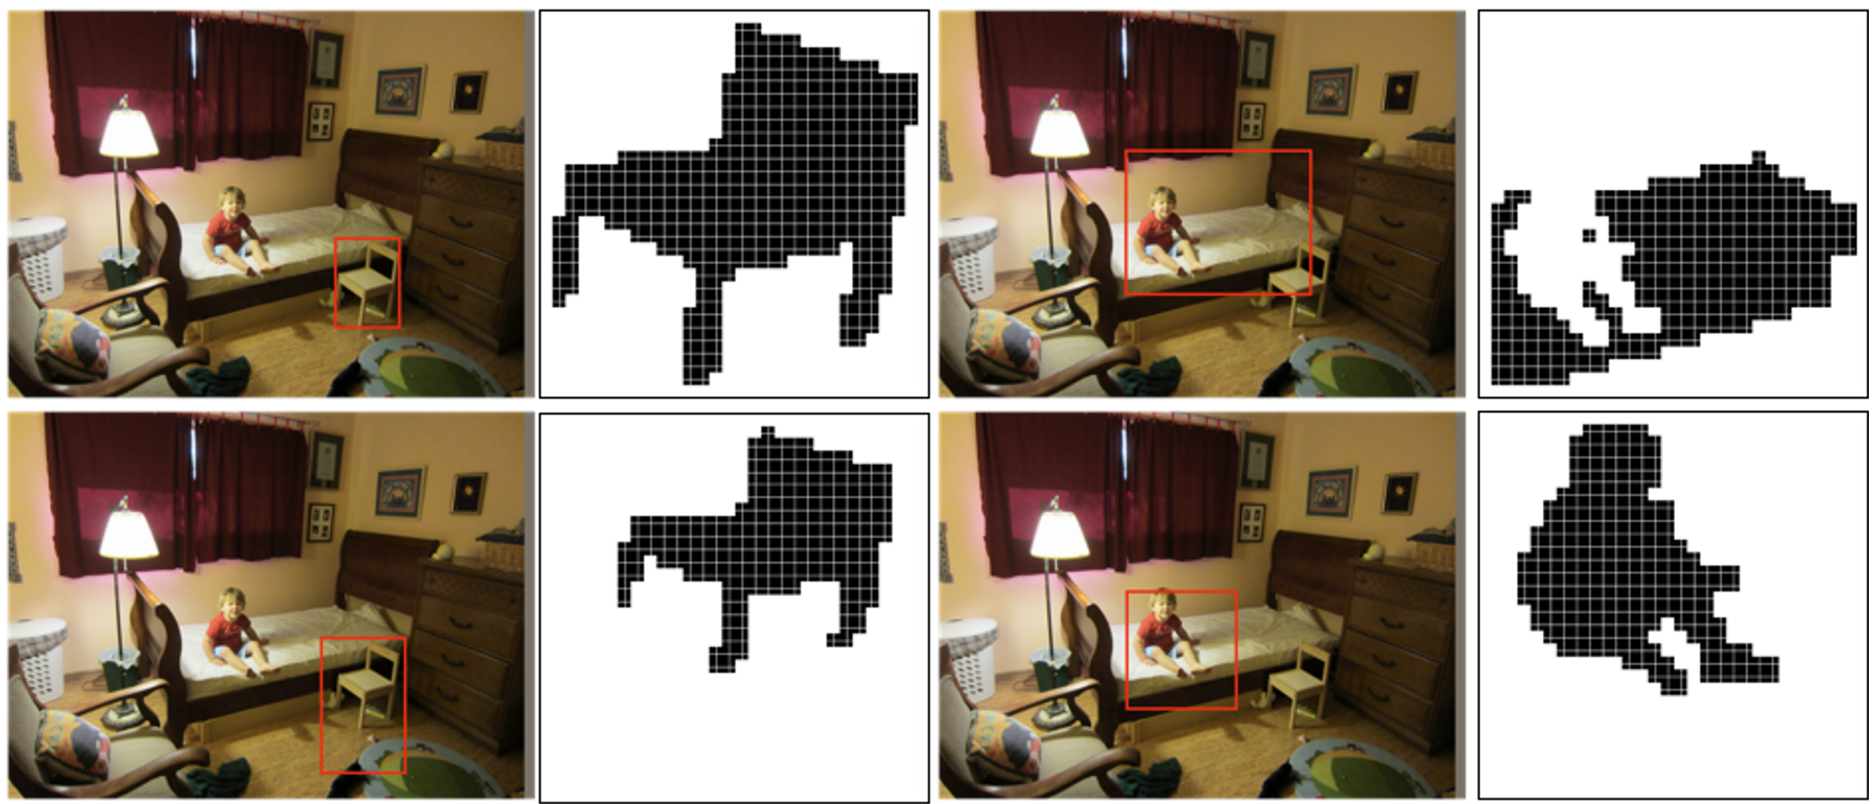
\includegraphics[width=1.0\textwidth,height=1.0\textheight,keepaspectratio]{images/object-detect/ins_8.png}
        \end{figure}
    }
\end{frame}

\begin{frame}{Mask R-CNN: Very Good Results!}
    \begin{figure}
        \centering
        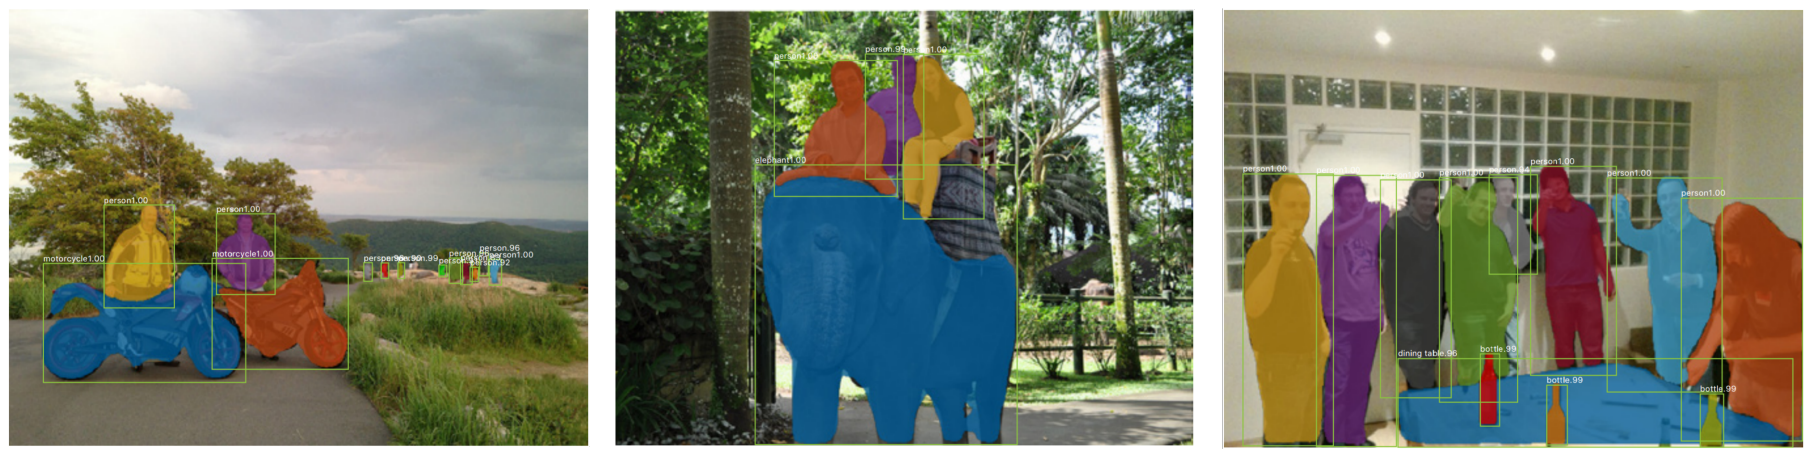
\includegraphics[width=1.0\textwidth,height=1.0\textheight,keepaspectratio]{images/object-detect/ins_9.png}
    \end{figure}
\end{frame}